% English master manuscript. Target: exactly six pages including references.
\documentclass[conference]{IEEEtran}
\IEEEoverridecommandlockouts
\usepackage{fontspec}
\setmainfont{Times New Roman}
\setsansfont{Arial}
\setmonofont{DejaVu Sans Mono}
\usepackage{graphicx}
\graphicspath{{figures/}{../../report/assets/}}
\usepackage{amsmath,amssymb}
\usepackage{booktabs}
\usepackage{array}
\usepackage{url}
\usepackage{balance}
\usepackage{microtype}

\title{Precision--Recall Trade-offs in Radar-Only, Camera-Gated, and Emergency-Fallback AEB: A Repeatable CARLA Study}

\author{
\IEEEauthorblockN{Mai Viet Hoang and Duc An Pham}
\IEEEauthorblockA{\textit{Hanoi University of Science and Technology}\\
Hanoi, Vietnam\\hoangmai04222@gmail.com}
}

\begin{document}
\maketitle

\begin{abstract}
A hard camera permission gate can suppress radar-triggered false braking, but it
can also veto genuine hazards outside the camera detector's label space. This
paper quantifies that trade-off and evaluates a conservative radar emergency
fallback in a sensor-to-brake automatic emergency braking (AEB) pipeline in
CARLA 0.9.11. Radar detections are path-filtered, clustered, tracked, and used
for time-to-collision and stopping-margin decisions; YOLO26n supplies \emph{car}
confirmation. The fallback permits an unconfirmed radar brake only for a
persistent, well-supported central track with simultaneously critical TTC and
stopping margin, then latches until radar brake release. A frozen GPU campaign
contains 2,461 runs in 639 process-isolated CARLA sessions. On a constructed
525-run core benchmark excluding labelled synthetic faults, radar-only,
hard-gate, and fallback policies respectively obtain precision/recall of
0.913/0.988, 1.000/0.965, and 1.000/0.988; fallback reduces hard-gate collisions
from 25 to 15. This apparent combination does not generalize as dominance. On a
70-run frozen hold-out, fallback precision falls to 0.600 because convincing
6--10-point synthetic ghosts trigger 20 false brakes; all policies collide in
15 runs involving three unseen physical props. Ablation, perturbation, camera
disabling, and CUDA timing identify both useful constraints and unresolved
failure modes. The results support camera gating as false-positive suppression
and emergency fallback as a conditional trade-off, not as a general obstacle
solution or safety certification.
\end{abstract}

\begin{IEEEkeywords}
automatic emergency braking, camera--radar fusion, CARLA, false braking,
precision--recall, fault injection, hold-out evaluation
\end{IEEEkeywords}

\section{Introduction}
Automatic emergency braking is a closed-loop perception--decision--actuation
problem. Radar directly supplies range and radial velocity, but a selected
return need not be a genuine obstacle in the ego path. Camera semantics can
reject implausible radar targets, but a missed or out-of-label object is not
proof that the road is clear. AEB reviews consequently treat perception,
decision logic, and control as an interdependent chain \cite{yang2022aebreview}.
Radar--vision vehicle recognition and AEB-oriented association are established
ideas \cite{kim2013vehicle,hsu2015noise}; this study does not claim a new fusion
primitive.

Simulation enables repeatable near-collision experiments
\cite{dosovitskiy2017carla,kang2019testing}, yet two methodological traps remain.
First, simulator actor identity or perfect kinematics can turn an end-to-end AEB
test into an ideal-state controller test. Second, repeatedly confirming a rule
on scenarios used to design it can hide its failure boundary. We therefore use
CARLA radar points and RGB frames for online decisions, reserve actor truth for
scoring, freeze the policy before hold-out, and retain all unsuccessful cases.

Earlier work from this project found a clear asymmetry: hard camera gating
removed 40/40 false brakes on non-hazard edge props, but missed central box and
barrel hazards in 10/10 runs. The present work asks whether a radar emergency
fallback can recover the latter without discarding the former. Its contributions
are: (1) a fixed three-policy comparison---radar-only, hard camera gate, and
camera gate with emergency fallback; (2) component ablation and one-factor
sensitivity; (3) perturbation, detector-disabled, and frozen hold-out suites;
and (4) a resumable GPU protocol that logs active inference providers and starts
a fresh CARLA server for each named scenario. The central result is deliberately
negative as well as positive: fallback combines the two core metrics, but strong
radar ghosts and unseen physical props prevent a dominance claim.

\section{Related Work and Positioning}
Radar--camera AEB has been studied at recognition, association, decision, and
actuation levels. Kim and Song combine radar and vision for vehicle recognition
\cite{kim2013vehicle}; Hsu \emph{et al.} address radar/camera noise filtering
for AEB target selection \cite{hsu2015noise}. Bae \emph{et al.} estimate the
closest in-path vehicle through low-channel LiDAR projection and camera tracking
on a real vehicle \cite{bae2021cipv}. Zhang \emph{et al.} combine curved-road
target recognition, TTC, safety distance, and graded braking in
CarSim/Simulink \cite{zhang2023curved}. These studies establish that semantic
verification, path relevance, and staged intervention are not individually new.

CARLA has supported full autonomous-pipeline validation under protocol-derived
scenarios \cite{gomez2022carla}. Its value here is not merely visualization: a
fixed-tick sensor-to-actuator loop permits collision-inducing tests, complete
tick logs, and repeatable policy substitution. Its limitation is equally
important. Simulator radar abstractions, graphics, map geometry, and actor
catalogues define a synthetic domain, while a simulator can expose privileged
truth unavailable to a deployed AEB. This work therefore separates online
sensor information from offline outcome truth and reports both system success
and detector/radar failure modes.

Table~\ref{tab:positioning} states the resulting position. Relative to prior
work, the contribution is not a higher-capacity detector or probabilistic
tracker. It is a controlled comparison of three late-decision policies plus a
frozen adverse hold-out. In particular, the hold-out asks whether a rule created
to recover weakly classified objects also accepts a radar fault that has the
same rule-level attributes. This falsification-oriented evaluation distinguishes
the study from a demonstration on nominal examples.

\begin{table*}[t]
\caption{Positioning against representative in-path perception and AEB studies.}
\label{tab:positioning}
\centering
\scriptsize
\setlength{\tabcolsep}{4pt}
\begin{tabular}{p{0.13\textwidth}p{0.24\textwidth}p{0.24\textwidth}p{0.27\textwidth}}
\toprule
Study & Perception / association & Decision / control & Evaluation emphasis\\
\midrule
Kim and Song \cite{kim2013vehicle} & Radar--vision vehicle recognition & AEB-oriented target recognition & Sensor-fusion recognition\\
Hsu \emph{et al.} \cite{hsu2015noise} & Radar/camera noise filtering & AEB target selection & Noise-filter design\\
Bae \emph{et al.} \cite{bae2021cipv} & LiDAR projection and camera tracking & Closest in-path vehicle for AEB & Real-vehicle scenarios\\
Zhang \emph{et al.} \cite{zhang2023curved} & Curved-road hazardous-target selection & TTC, safety distance, graded braking & CarSim/Simulink\\
This work & CARLA point-to-track radar and YOLO permission gate & Radar-only, hard gate, emergency fallback; staged PID & 2,461 runs; ablation, degradation, perturbation, frozen hold-out\\
\bottomrule
\end{tabular}
\end{table*}

\section{System and Policies}
\subsection{Sensor-to-brake information boundary}
The evaluated system uses a Tesla Model 3 on Town04, an RGB camera and a
100-m forward radar at a 0.05-s sensor tick. CARLA radar is a point-detection
model, not a raw FMCW signal chain; virtual radar fidelity depends on model
level \cite{magosi2022radar}. Exact sensor transforms calibrate radar-to-image
projection, and map height supports road-ground rejection. Online braking does
not query actor ID, actor velocity, class ground truth, or ground-truth boxes.
Those quantities are used only to label and score runs.

Radar points are rejected by range, height, road-ground, and a predicted
constant-curvature path. Remaining points are clustered by spatial and velocity
proximity and associated across frames. A selectable track must be confirmed,
non-stale, and collision-relevant. For selected distance $d$ and radar relative
velocity $v_r<0$,
\begin{equation}
 v_c=-v_r,\qquad \mathrm{TTC}=d/v_c.
\end{equation}
With ego speed $v_e$ and $v_t=\max(0,v_e+v_r)$, the stopping model is
\begin{equation}
 d_{\rm req}=\max\!\left(d_0,v_et_r+\frac{v_e^2}{2a_e}-
 \frac{v_t^2}{2a_t}+d_0\right),\quad m=d-d_{\rm req},
\end{equation}
where $t_r=0.20$~s, $a_e=8$~m/s$^2$, $a_t=6$~m/s$^2$, and $d_0=1$~m are
simulation risk parameters. A staged PID maps risk to continuous CARLA brake
with soft, medium, hard, and emergency bounds. The controller and its binary
ablation have been evaluated separately; staged PID avoids five additional
collisions in a 330-run system-limit sweep.

YOLO26n was fine-tuned for one \emph{car} class using CARLA images. Its held-out
in-domain precision, recall, $\mathrm{mAP}_{50}$, and
$\mathrm{mAP}_{50:95}$ are 0.9919, 0.9642, 0.9940, and 0.9495. These detector
scores establish narrow in-domain suitability, not AEB safety. For target
camera coordinates $(X_c,Y_c,Z_c)$,
\begin{equation}
 u=f_xX_c/Z_c+c_x,\qquad v=f_yY_c/Z_c+c_y,\quad Z_c>0.
\end{equation}
The camera confirms a radar target when $(u,v)$ lies inside a YOLO car box; the
confirmation is held for 0.35~s of simulation time.

The online order is fixed: update the ego path, filter radar points, update
tracks, select one target, compute radar risk, infer the latest camera frame,
apply one of the three permission policies, actuate, and log the next simulator
state. Camera boxes cannot create kinematic risk without a radar target. Radar
remains the source of distance and relative velocity. This ordering matters:
the policies differ only at the late permission gate, while radar processing,
risk equations, staged PID, scenario control, and scoring remain paired.

\subsection{Three brake policies}
Radar-only passes the radar AEB decision directly. The hard gate permits
\texttt{BRAKE} only with current or held camera confirmation. The proposed
fallback policy is
\begin{equation}
 B_f=B_r\land(C\lor H\lor E_r),
\end{equation}
where $B_r$ is radar brake, $C$ is current confirmation, $H$ is confirmation
hold, and $E_r$ is emergency radar evidence. The latter requires a confirmed,
non-stale track with age and hit streak $\geq3$, at least six cluster points,
confidence $\geq0.70$, predicted-path offset $\leq0.65$~m,
$\mathrm{TTC}\leq1.10$~s, and $m\leq-2.0$~m. TTC and margin must both be
critical. Once accepted, fallback is latched until radar leaves \texttt{BRAKE}.
No actor type or scenario label is used. This rule limits radar override; it
cannot prove that a well-supported radar track is physically genuine.

\begin{table}[t]
\caption{Frozen emergency-fallback configuration.}
\label{tab:fallback}
\centering
\footnotesize
\begin{tabular}{lr}
\toprule
Condition & Value\\
\midrule
Track age / hit streak & $\geq3/3$ frames\\
Cluster points / confidence & $\geq6/0.70$\\
Absolute path offset & $\leq0.65$ m\\
TTC / stopping margin & $\leq1.10$ s / $\leq-2.0$ m\\
Risk relation & TTC AND margin\\
Release & Latch until radar non-BRAKE\\
\bottomrule
\end{tabular}
\end{table}

\section{Frozen Experimental Protocol}
The simulator runs synchronously at 0.05~s with physics control. The v1 policy
and evaluation protocol were tagged before hold-out. Hard gate and fallback use
the same ONNX model, 640-pixel input, 0.15-s simulation-time cadence, and a
required \texttt{CUDAExecutionProvider}; CPU fallback or inference error is a
technical hard stop. A master runner checkpoints every run, executes all
repetitions of one named scenario, terminates CARLA, then starts a fresh Town04
server. Algorithmic failures do not stop the campaign.

The 2,461-run campaign comprises: 22 smoke runs; 324 development
ablation/sensitivity runs; 1,665 core runs (555 per policy); 180 local
perturbation runs; 60 detector-disabled runs; and 210 hold-out runs. Core
contains a repeated 66-case CCRm/CCRb/cut-in system-limit sweep, a mixed
vehicle/negative regression suite, 40 edge-prop runs, 10 central box/barrel
hazards, and 30 explicitly labelled four-point synthetic radar faults. The
faults are injections, not native CARLA ghost statistics.

Twenty perturbation conditions change ego speed by $\pm2$~km/h, gap by
$\pm1$~m, cut-in start by $\pm0.1$~s, and box lateral position by
$\pm0.15$~m. Detector-disabled tests emulate no camera detections. The frozen
hold-out contains new shopping-cart/bench/traffic-warning props, four vehicle
appearances, two edge props, and five persistent synthetic ghosts with 6--10
points. Hold-out results are not used to retune v1.

A positive label means braking is expected; a positive prediction means brake
was activated. Collision and full scenario PASS are reported separately because
a true-positive brake can still occur too late. Precision/recall are
composition-dependent: suite class ratios are deliberately designed, not road
prevalence. Wilson intervals describe run-level proportions, while
all-PASS/all-FAIL/mixed outcomes are also inspected by named scenario. Repeats
measure consistency and are not treated as independent traffic encounters.

\section{Results}
\subsection{Core trade-off}
Table~\ref{tab:main} excludes synthetic fault injection from the primary core
confusion matrix. Radar-only has higher recall than hard gate but 40 edge-prop
false brakes. Hard gate has no false positives but misses ten central
non-vehicle runs in addition to five late cut-out runs. Fallback recovers the ten
central runs while retaining zero core false positives. Its 15 collisions equal
radar-only and are ten fewer than hard gate. The 95\% Wilson intervals are
0.884--0.936 for radar precision, 0.973--0.995 for radar/fallback recall,
0.943--0.979 for hard-gate recall, and 0.991--1.000 for both zero-FP precision
estimates. Adding the 30 weak synthetic faults changes radar precision to 0.857;
both camera policies block all 30.

\begin{table}[t]
\caption{Core benchmark excluding synthetic fault injection (525 runs/policy).}
\label{tab:main}
\centering
\footnotesize
\setlength{\tabcolsep}{3pt}
\begin{tabular}{lrrrrrrr}
\toprule
Policy & TP & FP & TN & FN & Prec. & Rec. & Coll.\\
\midrule
Radar-only & 420 & 40 & 60 & 5 & .913 & .988 & 15\\
Hard gate & 410 & 0 & 100 & 15 & 1.000 & .965 & 25\\
Fallback & 420 & 0 & 100 & 5 & 1.000 & .988 & 15\\
\bottomrule
\end{tabular}
\end{table}

Across all 555 core runs, fallback improves 70 radar-only system outcomes and
regresses none; it improves ten hard-gate outcomes and regresses none. This is a
within-core statement. The frozen hold-out reverses the hard-gate comparison.
Fig.~\ref{fig:stress} isolates three deliberately constructed stresses. Radar
passes the central props but brakes on every edge prop and weak synthetic fault;
hard gate has the opposite central-prop outcome; fallback passes all three core
stress families.

\begin{figure}[t]
\centering
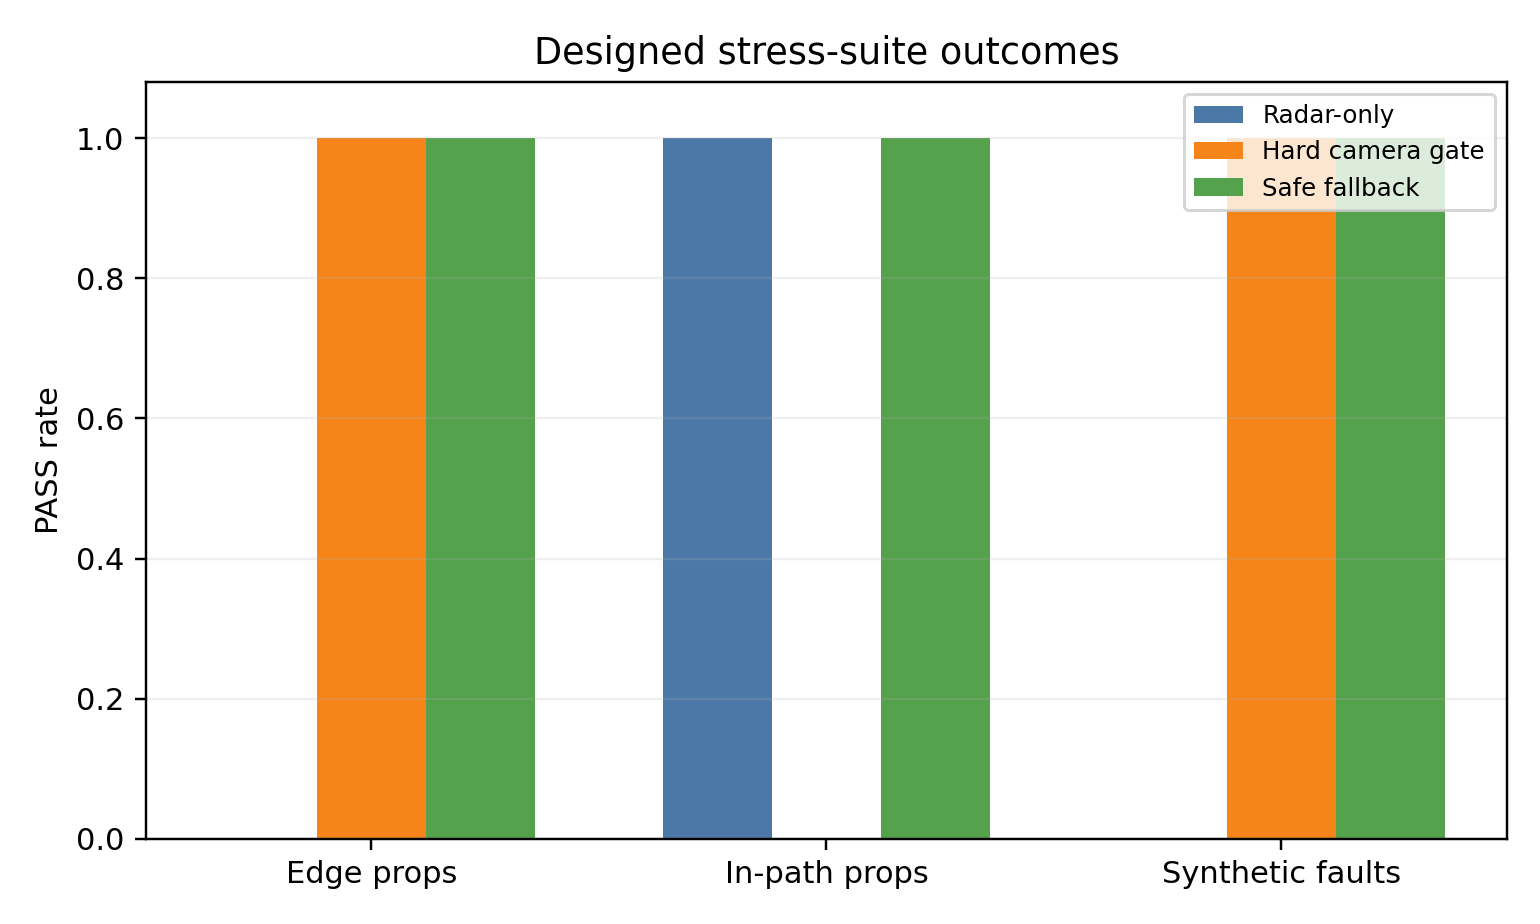
\includegraphics[width=0.98\columnwidth]{stress_suite_pass_rates.png}
\caption{Core stress-suite PASS rates. These suites are balanced mechanisms,
not a prevalence-weighted sample.}
\label{fig:stress}
\end{figure}

\begin{figure*}[t]
\centering
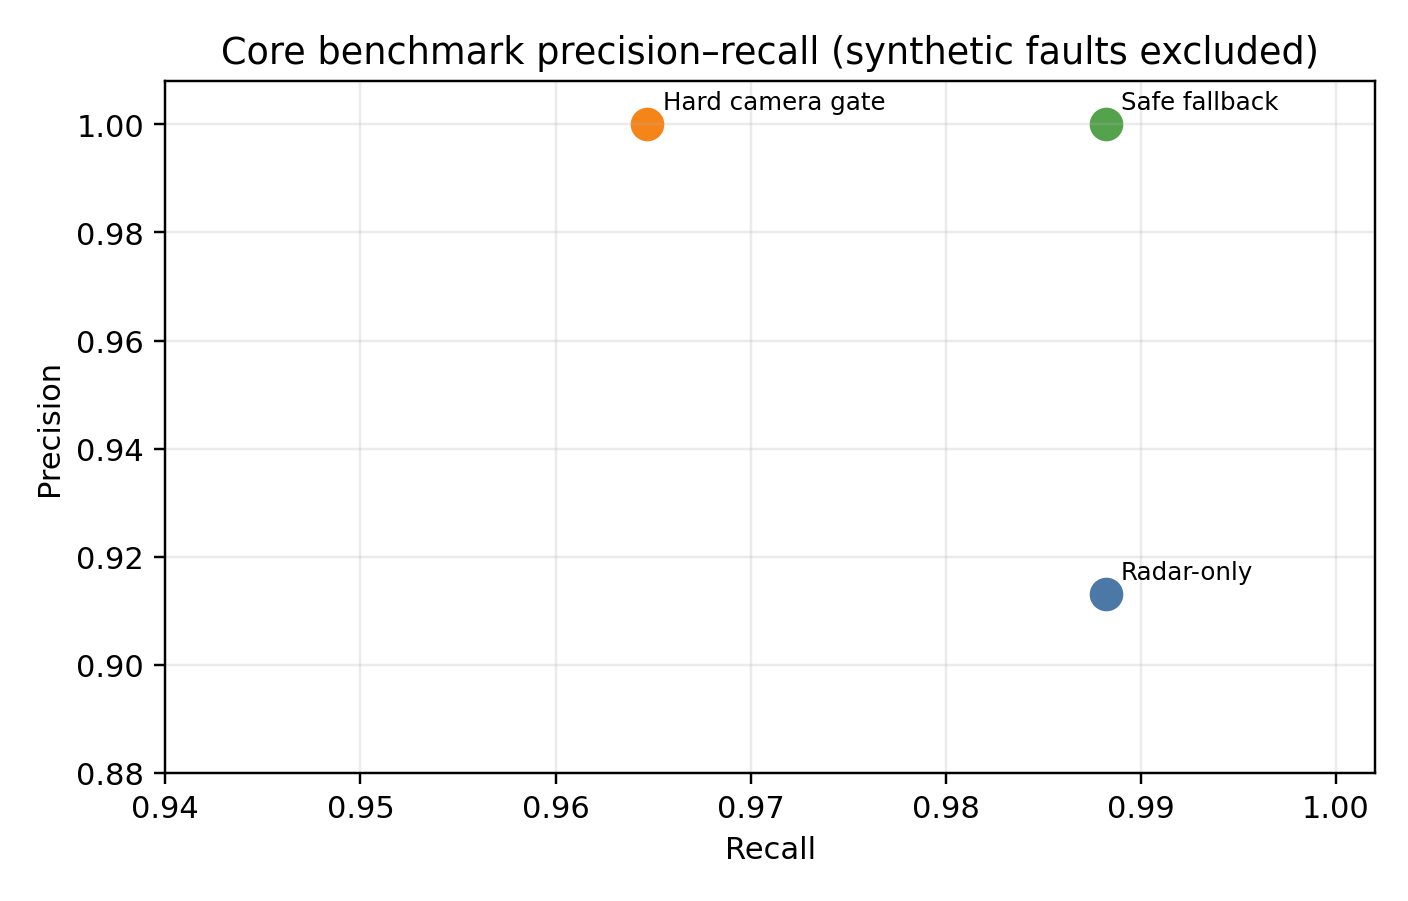
\includegraphics[width=0.47\textwidth]{core_precision_recall.png}\hfill
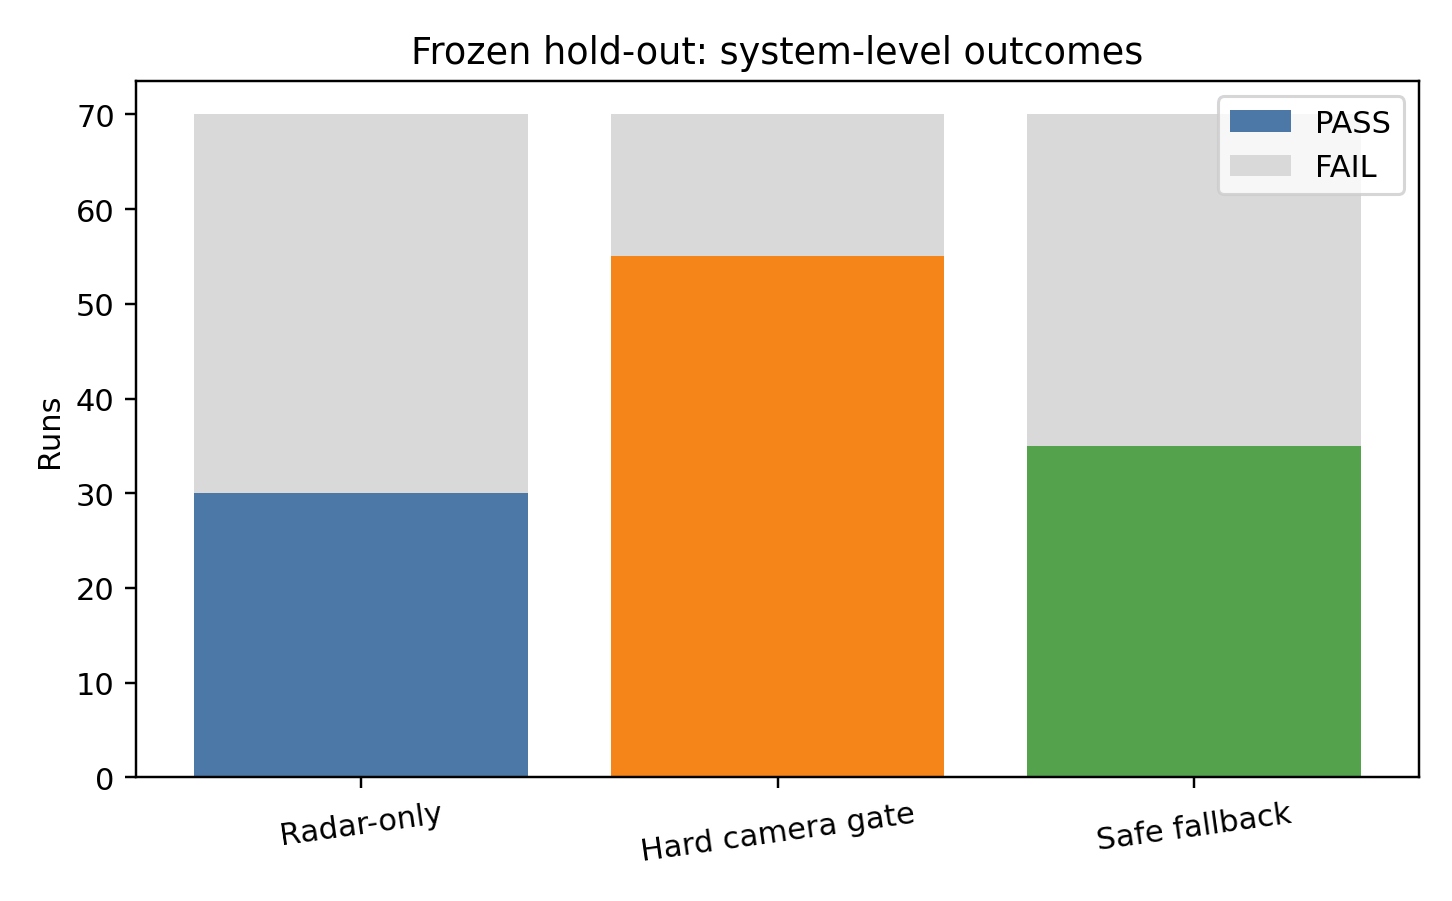
\includegraphics[width=0.47\textwidth]{holdout_pass_fail.png}
\caption{Left: core precision--recall with synthetic faults excluded. Right:
system-level PASS/FAIL on the frozen hold-out. Designed class ratios preclude
road-prevalence interpretation.}
\label{fig:tradeoff}
\end{figure*}

\subsection{Ablation, sensitivity, and degradation}
Fig.~\ref{fig:ablation} visualizes system-level PASS rates for the component
removals. It should not be read as equal statistical evidence for every rule:
the focused scenarios are designed to expose path, point-count, and latch
mechanisms, whereas all tracks are persistent and strongly critical.

\begin{figure}[t]
\centering
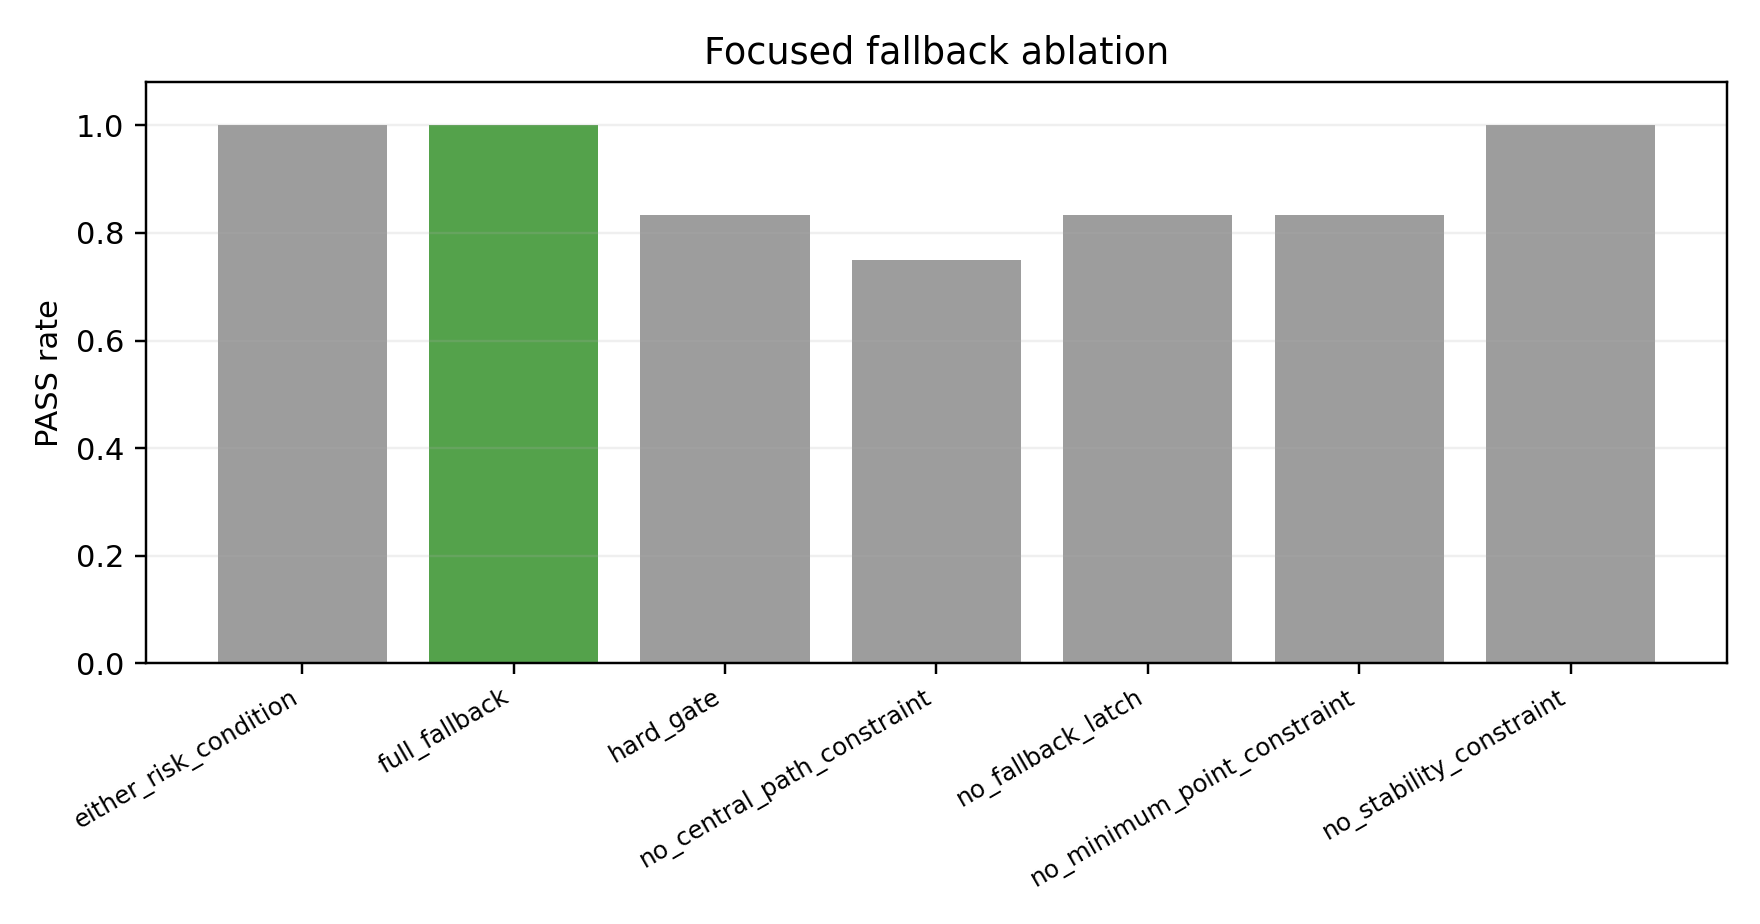
\includegraphics[width=0.98\columnwidth]{fallback_ablation.png}
\caption{Focused ablation. Full fallback passes 24/24; removing central-path,
point-count, or latch constraints creates the indicated failures.}
\label{fig:ablation}
\end{figure}
The focused ablation uses 12 development scenarios repeated twice. Full
fallback passes 24/24. Hard gate and no-latch each fail four central box/barrel
runs; removing the central-path constraint creates six edge-prop false brakes;
removing the point threshold creates four weak synthetic false brakes. Removing
stability/confidence or changing TTC-and-margin to TTC-or-margin does not change
this focused subset, so independent necessity is not claimed for those rules.

One-factor sensitivity uses six representative scenarios repeated twice. The
nominal policy passes 12/12. Reducing minimum points from six to four creates two
synthetic false brakes. Increasing stability from three to four frames or
tightening TTC from 1.10 to 0.90~s misses the central box twice. Tested path,
margin, confidence, and permissive-TTC alternatives do not change this subset.
These results expose a local precision--recall surface rather than optimize it.

\begin{table}[t]
\caption{Robustness and frozen hold-out outcomes.}
\label{tab:extended}
\centering
\scriptsize
\setlength{\tabcolsep}{3pt}
\begin{tabular}{llrrrrrr}
\toprule
Suite & Policy & Pass/N & TP & FP & TN & FN & Coll.\\
\midrule
Perturb. & Radar & 57/60 & 60 & 0 & 0 & 0 & 3\\
 & Hard & 45/60 & 45 & 0 & 0 & 15 & 15\\
 & Fallback & 54/60 & 60 & 0 & 0 & 0 & 6\\
\midrule
Camera off & Hard & 12/30 & 0 & 0 & 12 & 18 & 18\\
 & Fallback & 24/30 & 18 & 0 & 12 & 0 & 6\\
\midrule
Hold-out & Radar & 30/70 & 30 & 25 & 10 & 5 & 15\\
 & Hard & 55/70 & 25 & 0 & 35 & 10 & 15\\
 & Fallback & 35/70 & 30 & 20 & 15 & 5 & 15\\
\bottomrule
\end{tabular}
\end{table}

In perturbation tests, hard gate misses all five box conditions; fallback
recovers three, but collisions remain at 19- and 21-m gaps despite passing the
20-m nominal condition. Radar-only also collides at 19~m. This non-monotonic
outcome reflects return geometry, track confirmation time, and stopping margin.
With the detector disabled, fallback activates on all 18 positives but still
collides in six stationary/braking-lead runs because emergency evidence arrives
too late. Brake recall therefore does not imply safe stopping.

\subsection{Frozen hold-out and computational evidence}
Hold-out is the decisive non-dominance result. All policies collide in 15 runs
covering three new central props. The shopping cart produces at most two path
candidates and no confirmed target; bench and warning props trigger too late.
Fallback activates on four convincing central/0.50-m-offset ghosts, producing
20 false brakes, and blocks only the 0.75-m-offset ghost. Thus its hold-out
precision/recall are 0.600/0.857 versus hard gate's 1.000/0.714. In paired system
status, hard gate alone passes 20 runs, fallback alone passes none, both pass 35,
and both fail 15. The fallback recovers some brake labels but does not solve
unknown-obstacle detection.

The campaign records 474 CUDA sessions, 74,928 inferences, and zero inference
errors. Session-median p50/p95 are 9.95/11.53~ms and weighted mean is 11.56~ms.
Each isolated process has one cold start above 150~ms; the maximum is 276.10~ms.
These wall-clock measurements establish steady-state throughput on the tested
GPU while disclosing startup cost. Because synchronous simulation waits for
processing, they do not prove an automotive ECU deadline.

\subsection{Failure-mechanism decomposition}
The hold-out physical failures are not one homogeneous camera-gate effect. The
shopping cart yields at most two in-path candidates and no confirmed cluster,
so no policy brakes. The bench produces confirmed radar tracks: radar-only first
brakes at a 12.62-m bumper gap, fallback waits for emergency evidence until
4.30~m, hard gate never brakes, and all collide. The traffic-warning prop causes
a brake at 21.87~m even under hard gating, indicating apparent camera
confirmation, yet all policies still record collision. These cases separate
missing track, late emergency qualification, and collision/dynamics behavior.

The ghost results isolate a different mechanism. A six-point central injection
reaches one confirmed cluster and triggers radar-only/fallback at 0.15~s, whereas
hard gate blocks it. Eight- and ten-point central ghosts behave similarly. At a
0.75-m injected offset, radar-only still brakes but fallback rejects the track by
its 0.65-m path criterion. The expected precision loss is therefore a direct
consequence of fallback evidence, not YOLO timing.

The system-limit collisions are retained separately from perception trade-offs.
All policies brake in the 15 repeated failures associated with CCRb 95/110~km/h
at 20~m and the shortest high-speed cut-in; available distance is insufficient
under the configured dynamics. The regression suite adds five no-brake late
cut-outs at a lateral-corridor timing boundary. Conflating these with prop/ghost
outcomes would obscure which component can plausibly be improved.

\subsection{Traceability and statistical interpretation}
Every child run records the Git commit, seed, model and configuration SHA-256,
CARLA client/server version, fixed step, configured and active providers, and
per-tick gate reasons. The complete archive includes raw CSV, JSON summaries,
generated configuration snapshots, campaign/session manifests, and a SHA-256
sidecar. Re-running the analysis script regenerates the confusion, paired,
scenario-consistency, ablation, sensitivity, and timing tables. This traceability
is necessary because a scalar score cannot reveal whether a true-positive brake
was camera-confirmed, fallback-triggered, or too late.

Run-level Wilson intervals quantify finite counts but do not make repeated runs
independent. Scenario-level outcomes are therefore retained. The full66 core
sweep has 63 all-PASS and three all-FAIL named scenarios for each policy; the
mixed regression boundary is replaced by five consistent failures under fresh
server isolation. In perturbation, each failed named condition fails all three
repeats. In hold-out, every named condition is consistently all-PASS or all-FAIL.
This consistency strengthens attribution to configured boundaries while reducing
the effective independent sample size relative to the run count.

System-level paired comparisons also differ from brake confusion. On core,
fallback versus hard gate has 525 both-PASS, ten fallback-only PASS, and 20
both-FAIL runs. On hold-out, it has 35 both-PASS, zero fallback-only PASS, 20
hard-only PASS, and 15 both-FAIL. Reporting both matrices prevents the additional
fallback true-positive brakes in already-colliding prop cases from being
misrepresented as safety improvements.

\begin{figure}[t]
\centering
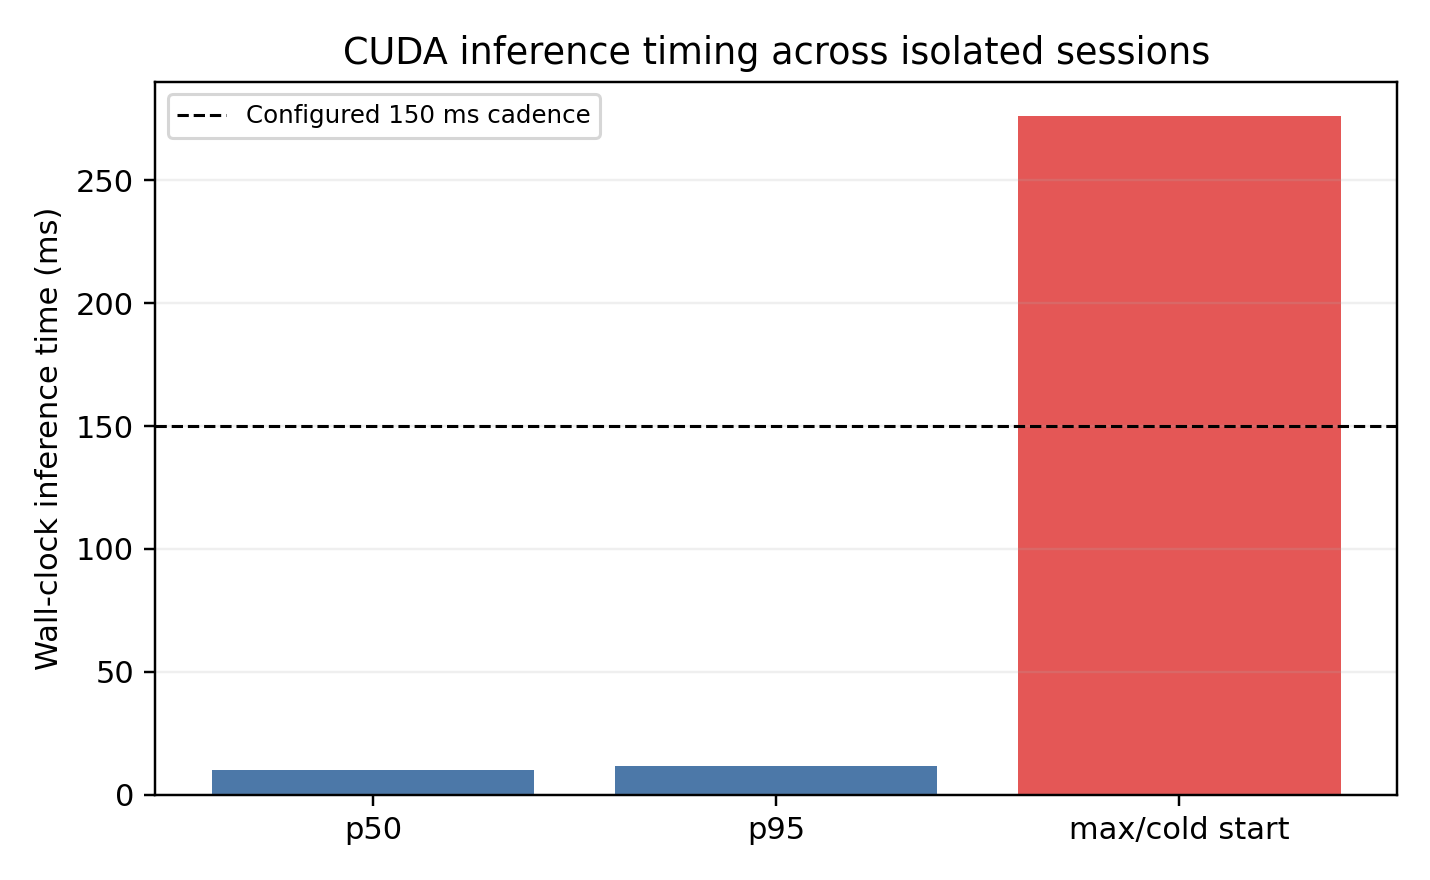
\includegraphics[width=0.96\columnwidth]{gpu_inference_latency.png}
\caption{CUDA processing: steady-state p50/p95 versus one disclosed cold-start
outlier in each isolated detector process.}
\label{fig:latency}
\end{figure}

\section{Discussion and Limitations}
\subsection{Design implications}
The three policies correspond to different error costs rather than a strict
ranking. Radar-only is appropriate as a diagnostic upper bound on radar hazard
recall, but its responses to every designed edge prop and synthetic fault make
it unsuitable when unnecessary braking is costly. Hard gating is the most
conservative about unverified radar objects and has the highest hold-out system
PASS count, but its car-only semantics make non-vehicle recall structurally
limited. Emergency fallback deliberately moves toward radar recall and should be
selected only if the operational design domain and downstream controller can
tolerate its high-support-ghost failure mode.

The fallback conditions also suggest where rule tuning reaches diminishing
returns. Point count, confidence, persistence, path offset, TTC, and stopping
margin are all attributes of the estimated track; none is independent evidence
that an object exists. Increasing their thresholds rejects weak faults but also
consumes stopping distance. A qualitatively new evidence source is needed to
break this symmetry: calibrated free-space estimates, broader obstacle
semantics, radar cross-section or temporal micro-Doppler cues, multi-sensor
existence probability, or map-independent occupancy. Until then, tuning shifts
the operating point rather than eliminating the trade-off.

Evaluation should consequently report more than brake confusion. A policy may
produce a true-positive brake yet collide because target formation or permission
arrives too late. Conversely, a false brake has severity dimensions---onset
speed, duration, deceleration, and traffic context---that a binary FP count does
not capture. This study reports collision, first brake, minimum gap, and gate
reason in raw logs, but its headline tables remain binary for comparability.
Future campaigns should pre-register impact speed, residual stopping margin,
brake duration, and jerk-aware cost, then aggregate by named condition before
run-level totals.

\subsection{Validity boundaries}
The evidence supports a narrower conclusion than ``fusion is better.'' Camera
gating is effective false-positive suppression when the detector label space
covers the intended hazard. Radar fallback can recover selected out-of-label
objects, but any rule that accepts a stable, central, high-support radar track is
also vulnerable to a stable, central, high-support ghost. Raising quality or
risk thresholds then delays or suppresses genuine-object braking, as sensitivity
and camera-off results demonstrate.

External validity remains limited by one map and ego vehicle, favorable imaging,
a one-class detector, and point-level CARLA radar. Synthetic ghosts are explicit
fault models rather than measured multipath distributions. The hold-out adds
appearance and prop diversity but is small and deliberately balanced. No
hardware-in-the-loop, actuator/communication delay, tire-friction sweep, real
sensor data, or vehicle test is included. The CCR families are inspired by AEB
testing but do not reproduce Euro NCAP apparatus or certify compliance
\cite{euroncap_aeb}. Future work should prioritize uncertainty-aware tracking,
free-space or multi-class visual evidence, time-varying sensor degradation,
recorded radar/camera data, and impact-speed/stopping-margin objectives before
expanding nominal repeat counts.

\section{Conclusion}
A conservative radar emergency fallback combines hard-gate precision and
radar-only recall on the constructed core benchmark, but frozen hold-out results
show that this combination is not general. Strong radar ghosts trade precision
for recall, while some unseen physical obstacles are not tracked early enough by
any policy. The main engineering outcome is therefore a reproducible map of
trade-offs and failures: camera gating suppresses false brakes; emergency
fallback conditionally restores obstacle recall; neither is a general safety
solution. All claims are confined to synchronous CARLA simulation and do not
constitute NCAP, functional-safety, real-time deployment, or real-vehicle
validation.

\balance
\bibliographystyle{IEEEtran}
\bibliography{references}
\end{document}
